\documentclass[margin=0.1cm]{standalone}
\usepackage{ tikz }
\usepackage{ xparse }
\usepackage{../../../macros}

\begin{document}
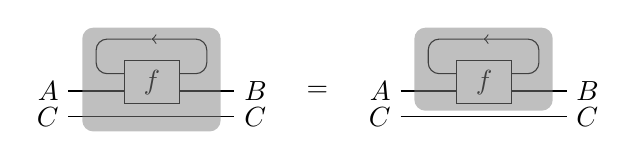
\begin{tikzpicture}[yscale=-1,x=1em,y=1.25em]

    \node [anchor=east] at (0,-0.25) {$C$};
    \node [anchor=east] at (0,-1) {$A$};
    \node [anchor=west] at (6,-0.25) {$C$};
    \node [anchor=west] at (6,-1) {$B$};

    \draw (0,-0.25) -- (6,-0.25);
    \draw (0,-1) -- (2,-1);
    \node[draw, minimum height = 1.5em, minimum width = 2em, anchor = west] at (2,-1.25){$f$};
    \draw (4,-1) -- (6,-1);
    \draw [->, rounded corners] (4,-1.5) -- (5,-1.5) -- (5,-2.5) -- (3,-2.5);
    \draw [rounded corners] (3,-2.5) -- (1,-2.5) -- (1,-1.5) -- (2,-1.5);
    \node[rounded corners, fill=gray, minimum width = 5em, minimum height = 3.75em, opacity=0.5] at (3,-1.33) {};

    \node at (9,-1) {$=$};

    \node [anchor=east] at (12,-0.25) {$C$};
    \node [anchor=east] at (12,-1) {$A$};
    \node [anchor=west] at (18,-0.25) {$C$};
    \node [anchor=west] at (18,-1) {$B$};

    \draw (12,-0.25) -- (18,-0.25);
    \draw (12,-1) -- (14,-1);
    \node[draw, minimum height = 1.5em, minimum width = 2em, anchor = west] at (14,-1.25){$f$};
    \draw (16,-1) -- (18,-1);
    \draw [->, rounded corners] (16,-1.5) -- (17,-1.5) -- (17,-2.5) -- (15,-2.5);
    \draw [rounded corners] (15,-2.5) -- (13,-2.5) -- (13,-1.5) -- (14,-1.5);
    \node[rounded corners, fill=gray, minimum width = 5em, minimum height = 3em, opacity=0.5] at (15,-1.63) {};

\end{tikzpicture}
\end{document}